%%%%%%%%%%%%%%%%%%%%%%%%%%%%%%%
% CHAPTER 4: EXPLORATORY STUDY
% 	RESULTS 3 - Results: Analysis of folder overlap
% File: tex/expstudy-chapter/expstudy-results3-folder-overlap.tex
%%%%%%%%%%%%%%%%%%%%%%%%%%%%%%%%%%%%%%%%%%%%%%%%
%%%%%%%%%%%%%%%%%%%%%%%%%%%%%%%%%%%%%%%%%%%%%%%%
%%%%%%%%%%%%%%%%%%%%%%%%%%%%%%%%%%%%%%%%%%%%%%%%
%%%%%%%%%%%%%%%%%%%%%%%%%%%%%%%%%%%%%%%%%%%%%%%%%%%%
%%%%%%%%%%%%%%%%%%%%%%%%%%%%%%%%%%%%%%%%%%%%%%%%%%%%
\newpage
\section{Results: Analysis of Folder Overlap}
\label{exp-study:Results-folder-overlap}
%%%%%%%%%%%%%%%%%%%%%%%%%%%%%%%%%%%%%%%%%%%%%%%%%%%%
%%%%%%%%%%%%%%%%%%%%%%%%%%%%%%%%%%%%%%%%%%%%%%%%%%%%
% the extent of \textit{folder overlap} between collections (folders common to multiple collections) was investigated to explore the similarity of pairs of hierarchies for a particular user. The motivation and execution of this novel technique is discussed in detail in . % Results are reported in \textbf{Section~\ref{exp-study:Results-folder-overlap}}.
% An important objective at this stage was to develop appropriate methods for comparing the folder hierarchies to contrast how participants organized the three types of information. 
% Overlapping folders are defined as those that appear in more than one hierarchy.
% Overlapping folders are in turn analysed in terms of organizational dimensions.
% This novel technique was employed in the \textit{between-tools/within-user} analysis (see below).
%	\item Analysis of folder overlap (folders common to multiple collections).
This section describes the investigation of the extent of \textit{folder overlap} between collections to explore whether participants tended to create similar folders in different tool contexts. The motivation and method used in this analysis is discussed in \textbf{Section~\ref{exp-study:analysis-folder-overlap}}.

%%%%%%%%%%%%%%%%%%%%%%%%%%%%%%%%%%%%%%%%%%%%%%%%%%%%%%%%%%%%%%%%%%%%%%%
% EXPAND WITH EXAMPLES OF PEOPLE WITH HIGH AND LOW OVERLAPS
%%%%%%%%%%%%%%%%%%%%%%%%%%%%%%%%%%%%%%%%%%%%%%%%%%%%%%%%%%%%%%%%%%%%%%%
The amount of overlap varied significantly between participants, and between collection pairs:
\begin{itemize}
\item Of all the participants, the highest overlap was observed for P13 who had 21 overlapping folders between his file and email collections, which had 60 and 85 folders respectively.  This was equivalent to 35\% of his file folders and 25\% of his email folders (he was one of the few participants with more file folders than email folders).  His file/email overlap mainly related to \textit{roles} (e.g. \texttt{General dept}, \texttt{Admin}, \texttt{Admin resp}, \texttt{Grading working-group}, \texttt{Course-planning}), and \textit{projects} (e.g. \texttt{Digital-library}, \texttt{LIDS}, and  \texttt{Niupapa}). However, since he had only 6 bookmark folders, the other overlaps were relatively smaller.  The \textit{file/bookmark} overlap was 1 folder (\texttt{Digital-library}), and the \textit{email/bookmark} overlap was 2 folders (\texttt{Digital-library} and \texttt{Conferences}).

\item In contrast, Participant P19 had much smaller overlaps between each pair of collections. Three folders overlapped between files and email (\texttt{Personal}, \texttt{Research}, \texttt{VB}), 2 between files and bookmarks (\texttt{Personal}, \texttt{414}), and 1 between email and bookmarks (\texttt{Personal}).
\end{itemize}

% \textit{Provide some examples of participants with high overlap and participants with low overlap.}
Rather than go through participants individually, aggregate results are presented as follows to provide an overview of the data (see \textbf{Table~\ref{table:category-overlaps}})\footnote{Note that Participant P5 who saved email messages as Word documents within the file structure was not included.}.
%%%%%%%%%%%%%%%%%%%%%%%
% INCLUDE DIAGRAM?
%%%%%%%%%%%%%%%%%%%%%%%
% \textbf{Figure~\ref{fig:exp-study:overlaps-per-user}} reports the overlap across all participants.
%\textit{Explain diagram. Note that the extent of category overlap varied enormously between users and between pairs of hierarchies. Explain reasons why. 
% %%%%%%%%%%%%%%%%%%%%%%%%%%%%%%%%%%%%%%%%%%%%
% FIGURE - OVERLAPS PER USER (FROM CORELDRAW?)
% %%%%%%%%%%%%%%%%%%%%%%%%%%%%%%%%%%%%%%%%%%%%
%\begin{figure}[t]
%	\begin{center}
%		\leavevmode
%		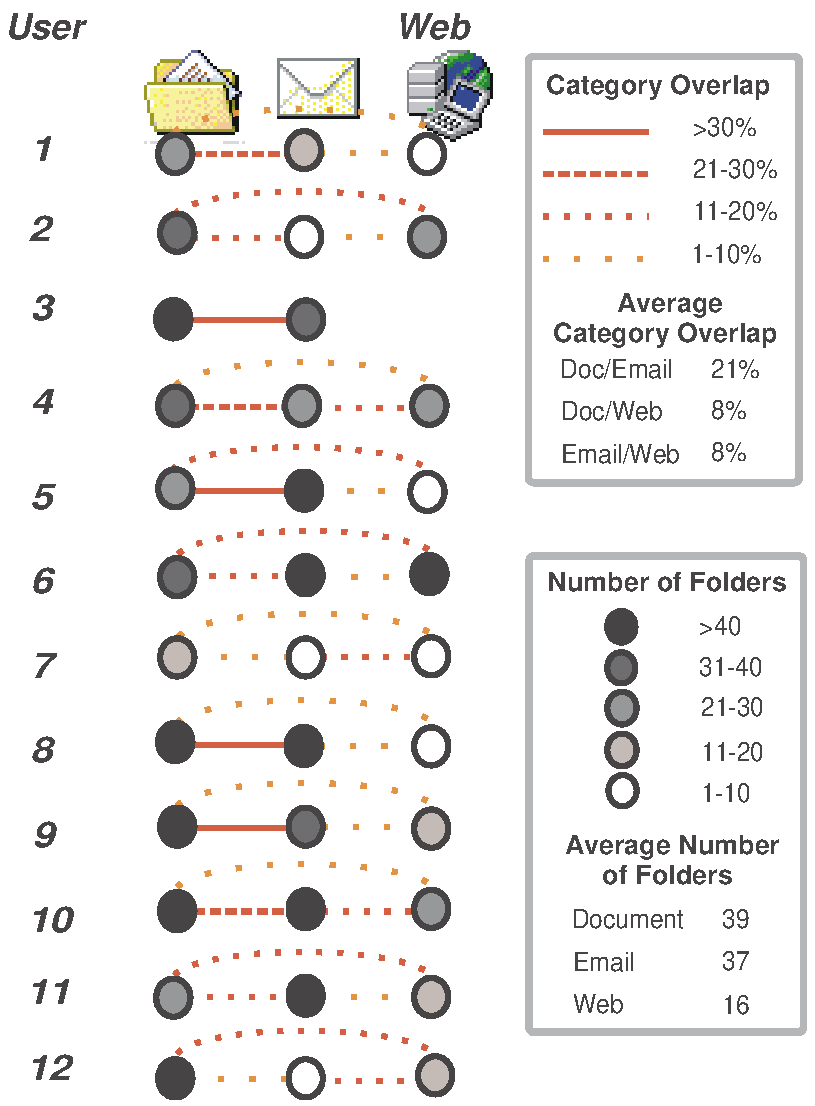
\includegraphics{pictures/exp-study/exp-study-OverlapResults.pdf}
%	\end{center}
%	\caption{Folder Overlaps for individual users [n=12]}
%	\label{fig:exp-study:overlaps-per-user}
%\end{figure}
Significant overlap was observed for many participants, particularly between files and email.   
For the twenty-two participants who had both file and email folders, the average \textit{file/email} overlap was 7.4 folders (SD: 4.6, min: 0, max: 21).
The other overlaps were consistently smaller.  For the eighteen participants with file and bookmark folders, the average \textit{file/bookmark} overlap was 2.6 folders (SD: 1.94, min: 0, max: 8).  Eighteen participants had created email and bookmark folders. The average \textit{email/bookmark} overlap was 2.0 folders (SD: 1.5, min: 0, max: 5).
% The file/web and email/web overlaps were on average almost three times smaller.
In other words, folder overlap was not distributed evenly between the hierarchy pairs\footnote{Overlaps were lower than previously estimated in~\citep{rpb:01a}. This is due to the earlier results being skewed upwards by the smaller number of subjects at that stage in the study.}.

%%%%%%%%%%%%%%%%%%%%%%%%%%%%%%%%%%%%%%%%%%%%%%%%%%%%%%
% TABLE: FOLDER OVERLAPS
% in tables/ch2/exp-study-tables.xls
%%%%%%%%%%%%%%%%%%%%%%%%%%%%%%%%%%%%%%%%%%%%%%%%%%%%%%
\begin{table}[hbp]
\begin{center}
\begin{footnotesize}
\setlength{\extrarowheight}{2pt}
\begin{tabular}{|p{4cm}|p{3cm}|p{3cm}|p{3cm}|}
% Table generated by Excel2LaTeX from sheet 'Folder Overlaps'
\hline
    {\bf } & {\bf File/email} & {\bf File/web} & {\bf Email/web} \\
\hline
{\bf \# participants with folders in corresponding tools} &         22 &         18 &         18 \\
\hline
{\bf Average overlap (\# of folders)} & 7.4 (SD: 4.6, min: 0, max: 21) & 2.6 (SD: 1.94, min: 0, max: 8) & 2.0 (SD: 1.5, min: 0, max: 5) \\
\hline
{\bf Average overlap as \% of file folders} & 16.3\% (SD:12.2\%, min: 0\%, max: 46.4\%) & 6.6\% (SD:5.4\%, min:0\%, max: 22.2\%) &        n/a \\
\hline
{\bf Average overlap as \% of email folders} & 21.6\% (SD:11.8\%, min:0\%, max: 40\%) &        n/a & 9.6\% (SD:10\%, min:0\%, max: 33\%) \\
\hline
{\bf Average overlap as \% of bookmark folders} &        n/a & 24.7\% (SD:17.2\%, min:0\%, max: 66.7\%) & 17.3\% (SD:12.4\%, min:0\%, max: 40\%) \\
\hline
\end{tabular}  
\end{footnotesize}
\caption{Folder overlaps between the three pairs of PIM-tools}
\label{table:category-overlaps}
\end{center}
\end{table}


Interestingly, as in the case of P19 above, the \textit{file/bookmark} and \textit{email/bookmark} overlaps tended to be a subset of the larger \textit{file/email} overlap. For the majority of subjects, the two smaller overlaps were almost identical. In other words, the subset they represented was common to all three tools.
%%%%%%%%%%%%%%%%%%%%%%%%%%%%%%%%%%%%%%%%%%%%
% EMPHASISE OVERLAP BETWEEN ALL 3 TOOLS
%%%%%%%%%%%%%%%%%%%%%%%%%%%%%%%%%%%%%%%%%%%%


%%%%%%%%%%%%%%%%%%%%%%%%%%%%%%%%%%%%%%%%%%%%%%
% Dimensional make-up of overlapping folders
%%%%%%%%%%%%%%%%%%%%%%%%%%%%%%%%%%%%%%%%%%%%%%
% Most overlapping folders were based on users' projects (40\%) or roles (27\%).
% RATIONALE: The purpose of this analysis was to see if overlapping folders tended to be based on a particular organizational dimensions . 
\textbf{Tables~\ref{table:file-email-overlap}}, \textbf{\ref{table:file-bookmark-overlap}}, and \textbf{\ref{table:email-bookmark-overlap}} show the organisational dimensions for the overlapping folders in each collection pair.  Interestingly, all three overlaps were predominantly based on the users' \textit{roles} and \textit{projects} (file/email: 75\%, file/bookmark: 79\%, email/bookmark: 79\%). This suggests that the dimensions of \textit{role} and \textit{project} are more likely to carry meaningful context across an entire workspace than other types of label. % Such overlap suggests that multiple types of information are involved in high-level user roles and activities.

%%%%%%%%%%%%%%%%%%%%%%%%%%%%%%%%%%%%%%%%%%%%%%%%%%%%%%
% TABLE: DIMENSIONS IN FILE/EMAIL OVERLAP (GROUP C USERS)
% in tables/ch2/exp-study-tables.xls
%%%%%%%%%%%%%%%%%%%%%%%%%%%%%%%%%%%%%%%%%%%%%%%%%%%%%%
\begin{table}[hbt]
\begin{center}
\begin{footnotesize}
\setlength{\extrarowheight}{2pt}
% Table generated by Excel2LaTeX from sheet 'File-EM O-Dims'
\begin{tabular}{|c|c|c|c|}
\hline
{\bf Rank} & {\bf Dimension in file/email folder overlap} & {\bf Count} &   {\bf \%} \\
\hline
   {\bf 1} &    Project &         60 &       36\% \\
\hline
   {\bf 2} &       Role &         59 &       36\% \\
\hline
   {\bf 3} &    Contact &         14 &        8\% \\
\hline
   {\bf 4} & Topic / interest &         13 &        8\% \\
\hline
   {\bf 5} & Document class &          5 &        3\% \\
\hline
   {\bf 6} &     Format &          5 &        3\% \\
\hline
   {\bf 7} &      Event &          4 &        2\% \\
\hline
   {\bf 8} &    General &          3 &        2\% \\
\hline
   {\bf 9} & Other (<3 folders) &          3 &        2\% \\
\hline
           & {\bf Total} &  {\bf 166} & {\bf 100\%} \\
\hline
\end{tabular}  
\end{footnotesize}
\caption{Organisational dimensions in file/email folder overlap [n=22]}
\label{table:file-email-overlap}
\end{center}
\end{table}

%%%%%%%%%%%%%%%%%%%%%%%%%%%%%%%%%%%%%%%%%%%%%%%%%%%%%%%
% TABLE: DIMENSIONS IN FILE/BOOKMARK OVERLAP (GROUP C USERS)
% in tables/ch2/exp-study-tables.xls
%%%%%%%%%%%%%%%%%%%%%%%%%%%%%%%%%%%%%%%%%%%%%%%%%%%%%%%
\begin{table}[hbt]
\begin{center}
\begin{footnotesize}
\setlength{\extrarowheight}{2pt}
% Table generated by Excel2LaTeX from sheet 'File-BM O-Dims'
\begin{tabular}{|c|c|c|c|}
\hline
{\bf Rank} & {\bf Dimension in file/bookmark folder overlap} & {\bf Count} &   {\bf \%} \\
\hline
   {\bf 1} &    Project &         17 &       41\% \\
\hline
   {\bf 2} &       Role &         11 &       27\% \\
\hline
   {\bf 3} & Topic / interest &          9 &       22\% \\
\hline
   {\bf 4} &    Contact &          2 &        5\% \\
\hline
   {\bf 5} & Other (<2 folders) &          2 &        5\% \\
\hline
    {\bf } &     {\bf Total} &   {\bf 41} & {\bf 100\%} \\
\hline
\end{tabular}  
\end{footnotesize}
\caption{Organisational dimensions in file/bookmark folder overlap [n=18]}
\label{table:file-bookmark-overlap}
\end{center}
\end{table}

%%%%%%%%%%%%%%%%%%%%%%%%%%%%%%%%%%%%%%%%%%%%%%%%%%%%%%%
% TABLE: DIMENSIONS IN EMAIL/BOOKMARK OVERLAP (GROUP C USERS)
% in tables/ch2/exp-study-tables.xls
%%%%%%%%%%%%%%%%%%%%%%%%%%%%%%%%%%%%%%%%%%%%%%%%%%%%%%%
\begin{table}[hbt]
\begin{center}
\begin{footnotesize}
% Table generated by Excel2LaTeX from sheet 'EM-BM O-Dims'
\begin{tabular}{|c|c|c|c|}
\hline
{\bf Rank} & {\bf Dimension in email/bookmark folder overlap} & {\bf Count} &   {\bf \%} \\
\hline
  {\bf 1=} &    Project &         11 &       35\% \\
\hline
  {\bf 1=} &       Role &         11 &       35\% \\
\hline
   {\bf 2} & Topic/interest &          5 &       16\% \\
\hline
   {\bf 3} & Document class &          2 &        6\% \\
\hline
   {\bf 4} & Other (<2 folders) &          2 &        6\% \\
\hline
    {\bf } & {\bf Total} &   {\bf 31} & {\bf 100\%} \\
\hline
\end{tabular}  

\end{footnotesize}
\caption{Organisational dimensions in email/bookmark folder overlap [n=18]}
\label{table:email-bookmark-overlap}
\end{center}
\end{table}


%%%%%%%%%%%%%%%%%%%%
\subsection{Discussion}
\label{exp-study:Results-folder-overlap-discussion}
%%%%%%%%%%%%%%%%%%%%
%%%%%%%%%%%%%%%%%%%%%%%%%%%%%%%%%%%%%%%%%%%%%%%%%%%%%%%%%%%%
% TO ADD: WHY WAS THIS DONE? WHAT IS THE MAIN CONCLUSION?
%%%%%%%%%%%%%%%%%%%%%%%%%%%%%%%%%%%%%%%%%%%%%%%%%%%%%%%%%%%%

%%%%%%%%%%%%%%%%%%%%%%%%%%%%%%%%%%%
% Highest between files and email
%%%%%%%%%%%%%%%%%%%%%%%%%%%%%%%%%%%

%%%%%%%%%%%%%%%%%%%%%%%%%%%%%%%%%%%%%%%%%%%%%%%%%%%%%%%%%%%%%%%%
% Provide examples of overlap
% Provide examples of non-overlap (tool-specific activities)
%%%%%%%%%%%%%%%%%%%%%%%%%%%%%%%%%%%%%%%%%%%%%%%%%%%%%%%%%%%%%%%%
% \textit{Provide examples of overlapping folders (cross-tool activity) and tool-specific activities. }
The observation of a significant partial folder overlap for most participants points to a subset of user activities that involve the management of multiple types of information.  Folder overlap indicates that the study participants were devoting effort towards organizing resources relating to the same production activity in multiple tools.  In other words, there are \textit{redundant} aspects to user's information management activity when viewed from a cross-tool perspective.  Most overlapping folders corresponded to \textit{roles} and \textit{projects}, suggesting that these concepts may be usefully shared between collections, as in~\citep{Kaptelinin:03}.

However, it should be emphasized that folder overlap was only partial: all collections contained many unique folders.  This suggests that: (1) some production tasks are supported by single PIM tools and may not necessarily benefit from increased integration; and (2) users may have different organizational needs in different tools. 
% what does it mean in the grand scale of things? Provide balanced view a la Andrew Monk}.
% PIM-support for particular production activities is distributed across multiple PIM-related tools
% Distributed in time? Inter-tool consistency
%%%%%%%%%%%%%%%%%%%%%%%%%%%
% Reasons for overlap
% Reasons for no overlap
%%%%%%%%%%%%%%%%%%%%%%%%%%%
Several factors may contribute towards the disparity in overlap between different pairs of tools.

\begin{itemize}

\item Firstly, the number of folders differed greatly between the tools.  Typically bookmark collections contained fewer folders, resulting in smaller overlaps. In general bookmark organisation was not seen as being of as high a priority as file and email organisation, with subjects often preferring to use search engines in preference to recording bookmarks.

\item The previous section outlined the organisational make-up of each hierarchy and it was noted that the file and email hierarchies were relatively similar, both being dominated by \textit{projects} and \textit{roles}. This may account for their higher overlap. In contrast, the majority of bookmark labels were based on  \textit{interests} that had little relevance outside the information-seeking context of the web.

\item Document and email folders also tended to be managed more consistently in an ongoing manner -- thus the folders might be expected to match to a greater extent.

\item The information stored in each hierarchy may also be a factor. The file system was used to manage the user's own documents, or those authored by colleagues or friends. Likewise the email folders were often used to store threads of communication in which the user had actively participated (the storing of mailing lists is an exception). Both the document and email folders convey ownership over the static resources archived within. On the other hand, bookmark folders are used to store references to remotely authored websites. 

\end{itemize}

%%%%%%%%%%%%%%%%%%%%%%%%
% Awareness of overlap
%%%%%%%%%%%%%%%%%%%%%%%%
Most participants were not aware of the often significantly high level of overlap between their hierarchies.  Some participants seemed surprised when their high level of folder overlap was pointed out, suggesting that they had not reflected on how they organized different types of information.  A few were more aware and actually performed ad-hoc synchronisation of organisational structure. One participant (P11) had spent a large amount of time synchronising her email and web hierarchies. However the amount of effort involved meant the structures had not been kept in full synchronization.
% ADD: sample of anecdotal observations   regarding folder overlap and what it might mean(pos: dmw, neg: mar)

%%%%%%%%%%%%%%%%%%%%%%%%%
% DESIGN IMPLICATIONS
%%%%%%%%%%%%%%%%%%%%%%%%%
Folder overlap was greatest between the file and email collections. This highlights the potential compatibility for integration of files and \textit{filed} email. Also both types of information are either self-created or assessed as having long-term value.  However complete unification between files and \textit{all} email (as pointed to by designs such as~\citep{Bellotti:03}) may lead to the disruption of more controlled items (e.g. files, tasks) by unprocessed email. In some cases it may be appropriate not to integrate, but to instead retain tool separation.  Further design implications are presented in \textbf{Section~\ref{exp-study:discussion:integration}}.

%%%%%%%%%%%%%%%%%%%%%%%%%%%%%%
% hint at WorkspaceMirror?
%%%%%%%%%%%%%%%%%%%%%%%%%%%%%%
The observation of folder overlap contributes to the design rationale for the development of the WorkspaceMirror prototype in \textbf{Chapter~\ref{chapter:design}}. % Evidence is also provided of the cross-tool nature of information management: as an activity that supports a user's production activities.

%%%%%%%%%%%%%%%%%%%%%%%%%%%%%%%%%%%%%%%%%%%
%% END RESULTS2-FOLDER-OVERLAP/CHAPTER 4 EXP STUDY
%%%%%%%%%%%%%%%%%%%%%%%%%%%%%%%%%%%%%%%%%%%


